\documentclass[twoside]{projektInzynierskiMS}
\usepackage{polski}
\usepackage{lmodern}
\usepackage{graphicx}
\graphicspath{ {images/} }
\usepackage[utf8]{inputenc}
\usepackage{amsmath}
%\drukJednostronny

%% tytuł promotor iautor (\title to komenda standardowa)
\title{FilmUpper}
\promotor{dr inż. Adam Zielonka}


%% każdy autor musi mieć 4 argumenty: imię nazwisko, nr albumu, procent wkładu, opis wkładu
\autor{Kamil Rutkowski}{112233}{55} {Struktura aplikacji, Algorytmika}
	
\autor{Jakub Rup}{112233}{45}	{Kodowanie i dekodowanie plików, Interfejs użytkownika, Algorytmika}

	
	


%% dedykacja mile widziana
\dedykacja{To jest\\dedykacja}
%\NumeryNaPoczatku
%% numeracja wzorów tu włączona typu (1.2.3), ta druga to typu (1.2), domyślnie typu (1)
%\subsectionWzory
% \sectionWzory  

%\rozdzialy


%\literowaNumeracjaDodatkow %% włączy numerację dodatków literami
%\rzymskaNumeracjaDodatkow  %%włączy numerację dodatków liczbami rzymskimi

%% wyłączenie wyjaśnień:
\bezWyjasnien

%% standardowe komendy \newtheorem  działają jak woryginale
\newtheorem{tw}{Twierdzenie}%[subsection]
\newtheorem{twa}{Twierdzenie}%[section]
\newtheorem{dd}{Definicja}%[subsection]

\begin{document}


FilmUpper jest aplikacją pozwalającą na poprawianie jakości obrazu w filmie, poprzez zwiększanie rozdzielczości oraz zwiększanie ilości klatek na sekundę w nim występujących. Dzięki takim zabiegom jakość oglądanego przez nas obrazu znacząco się poprawia, jednakże nigdy nie będzie ona tak dobra, jak jakość obrazu nagrywanego z ustawieniami na które chcemy dany film skonwertować. 



\section{Technologia i język programowania}


Przetwarzanie plików filmowych nawet w przypadku zastosowania najłatwiejszych algorytmów sposób jest zadaniem bardzo wymagającym pod względem wydajnościowym, dlatego wybór technologii ma kluczowe znaczenie, gdyż wpływa na wydajność całej aplikacji. Należy zwrócić uwagę na wiele czynników które mogą wpłynąć na działanie programu jak również na sposób jego implementacji.

\subsection{Biblioteka do dekodowania oraz kodowania plików wideo}

\subsubsection{FFmpeg / libav}
Narzędzia oraz biblioteki \emph{FFmpeg} (czy też \emph{libav} będącym tak zwanym ,,forkiem'' \emph{FFmpeg}-a) są jednymi z najbardziej popularnych otwartych oprogramowań służących do dekodowania, kodowania oraz manipulacji plikami multimedialnymi. Posiadają one zbiór powszechnie używanych, ,,open-source'owych'' kodeków audio i wideo. Biblioteki te napisane są w języku C. 
\subsubsection{OpenCV}
\emph{OpenCV (Open Source Computer Vision)} to zbiór bibliotek napisanych w języku C++, przeznaczonych głównie do rozpoznawania obrazów w czasie rzeczywistym. Biblioteka \emph{cudacodec} zawarta w tym zbiorze pozwala na dekodowanie oraz kodowanie plików wideo. Jest ona oparta na kodekach \emph{FFmpeg}-a, do procesu przetwarzania multimediów używa karty graficznej.
\subsubsection{DirectShow}
Platforma programistyczna opracowana przez firmę \emph{Microsoft} dla systemów rodziny \emph{Windows}, przeznaczona do manipulacji plikami multimedialnymi. Oparta jest ona na standardzie \emph{Component Object Model (COM)}. Dzieli ona proces przetwarzania multimediów na moduły nazywane filtrami. Każdy filtr niezależnie wykonuje określone operacje na danych, przekazując je do kolejnego filtru, zapisując je lub wyświetlając na ekranie. Kodeki audio i wideo dostarczane są w formie takich filtrów.
\subsubsection{Media Foundation}
Następca \emph{DirectShowa} dostępny dla systemów \emph{Windows Vista} oraz nowszych. Działa na podobnej zasadzie co swój poprzednik, wspierając domyślnie większa liczbę formatów plików multimedialnych.
\subsubsection{Wybór biblioteki do dekodowania/kodowania}
Przy wyborze spośród narzędzi do dekodowania/kodowania kierowaliśmy się liczbą dostępnych pomocy naukowych na ich temat oraz prostotą ich używania. Początkowo wybraliśmy biblioteki \emph{FFmpeg}-a, jednakże ostatecznie przy tworzeniu projektu zastosowaliśmy rozwiązania oferowane przez \emph{OpenCV} do otrzymania danych z plików wideo oraz gotowych narzędzi \emph{FFmpeg}-a do późniejszego dodania dźwięku do otrzymanych plików multimedialnych.

\subsection{Biblioteka interfejsu graficznego}

\subsubsection{Qt}
\subsubsection{gtk}

\subsection{Język programowania}

Wybór właściwego języka programowania jest dla nas zadaniem kluczowym, ze względu na to, że użycie odpowiedniego języka znacząco wpływa na prędkość działania programu oraz na dostępność narzędzi i bibliotek wspomagających pracę nad przetwarzanymi danymi. Znajomość danego języka także była dla nas jednym z kluczowych czynników przy jego wyborze. Naszym rozważaniom poddaliśmy następujące języki programowania.

\subsubsection{C++}
Język C++ jest jednym z najczęściej używanych języków niskopoziomowych. Jego popularność jest skutkiem bardzo długiego czasu na rynku oraz pewnej prostoty użycia. Kolejne wersje tego wciąż rozwijającego się języka dodają nowe, sprawdzone i ułatwiające tworzenie programów rozwiązania z innych języków programowania. Bardzo duża wydajność oraz mnogość dostępnych bibliotek związanych z dekodowaniem i enkodowaniem plików filmowych jest bardzo ważnym aspektem tego wyboru. Wybór ten wiąże się także z kilkoma negatywnymi cechami tego języka, wymóg ręcznego zarządzania pamięcią, mało przejrzysta składnia przy tworzeniu rozwiązań o dużym stopniu skomplikowania, mało czytelne komunikaty odnośnie błędów podczas kompilacji i działania programu oraz brak ułatwień które poznaliśmy w językach wysokopoziomowych są jednymi z nich. 

\subsubsection{C\#}
Wysokopoziomowe rozwinięcie języka z rodziny C. Mimo posiadania składni podobnej do C++, język ten porzuca wiele z nieprzyjemnych jego aspektów. Poprzez automatyczne zarządzanie pamięcią, usunięcie składni charakterystycznej dla wskaźników oraz dodanie wielu nowych mechanizmów, wygląd kodu oraz prędkość tworzenia programów znacząco wzrasta. Bardzo ważnym składnikiem C\# jest także LINQ które umożliwia bardzo kompaktowe i przejrzyste działanie na kolekcjach co jest dużym plusem przy przetwarzaniu plików wideo, jako że są one kolekcjami pojedynczych klatek złożonych z kolekcji pikseli. Wszystkie z tych udogodnień mają jednak cenę w postaci mniejszej wydajności w stosunku do C++ oraz brak wystarczającego wsparcia dla zarządzania plikami wideo jako że język ten jest stworzony z myślą o szybkim tworzeniu aplikacji biurowych. 

\subsubsection{Rust}
Prędkość działania porównywalna z językiem C++, duże bezpieczeństwo pod względem zarządzania pamięcią, łatwość w konwersji programu jednowątkowego na wielowątkowy, składnia języka oraz wiele udogodnień zaciągniętych z języków wysokiego poziomu. To jedne z wielu punktów które zachęcały do wyboru tego języka. Niestety, z uwagi na to, że jest to język stosunkowo młody zauważalny jest brak lub wczesna wersja bibliotek umożliwiających przyjemną pracę na plikach filmowych. Jest to także język z którym nie mamy dużego doświadczenia.

\subsubsection{Python}
Python mimo bycia językiem wysokopoziomowym ma duże możliwości w przetwarzaniu ogromnych ilości danych dzięki bibliotece numpy. Jest to bardzo szybka biblioteka zaimplementowana w języku niskiego poziomu. Mieliśmy także styczności z tym językiem podczas naszych studiów. Dużym minusem jest dla nas brak silnych statycznych typów który znacząco ułatwia naukę nowych rozwiązań.

\subsubsection{Wybór języka programowania}
Rozważając cechy każdego z języków, nasze umiejętności w posługiwaniu się nimi oraz specyfikę programu który chcemy napisać wybraliśmy język C++. Kluczowymi cechami które przekonały nas do wyboru tego języka były: mnogość bibliotek związanych z tematem projektu lub uniwersalnie wspomagających często napotykane problemy, prędkość działania oraz duża znajomość samego języka.


\section{Dekodowanie oraz kodowanie filmów}

\subsection{Format pliku wideo}
Formatem pliku wideo nazywamy sposób reprezentacji danych wideo i audio w pamięci komputera. Na format wideo składa się kontener przechowujący strumienie między innymi audio i wideo oraz kodeki określające jak te strumienie są kodowane i kompresowane. Kontenery obsługują ściśle określone kodeki audio i wideo. Większość kontenerów jest w stanie przechowywać wyłącznie jeden strumień wideo oraz jeden strumień dźwięku, niektóre z nich mogą przechowywać informacje o napisach (przykładem kontenera pozwalającego na przechowywanie wielu strumieni takiego samego typu jest \emph{Matroska}).

\subsection{Struktura pliku wideo}
W pliku wideo wyróżnić można następujące elementy: 
\begin{itemize}
	\item nagłówek zawierający dane formacie pliku, jego kontenerze, zastosowanych kodekach oraz opcjonalne metadane takie jak tytuł czy też autor,
	\item pakiety posiadające dane o pewnych określonych częściach strumieni które są zapisane w pliku.
\end{itemize}
W przypadku strumienia wideo pojedynczy pakiet przechowuje dane o jednej jego klatce (bądź też, w przypadku niektórych kodeków, części która uległa zmianie względem poprzedniej klatki). Dla strumieni audio pakiet przechowuję dane o pewnej ilości próbek dźwięku zależnej od zastosowanego podczas kodowania próbkowania oraz ilości klatek wyświetlanych na sekundę. Pakiety przechowują także informacje pozwalające na synchronizacje czasową strumieni danych potrzebne do poprawnego odtwarzania pliku.

\subsection{Dekodowanie}
Aby odczytać z pliku wideo pojedynczą klatkę obrazu potrzebujemy wydobyć z niego pojedynczy pakiet i zdekodować go określonym przez format tego pliku kodekiem. Zanim do tego przystąpimy musimy jednak wydzielić pakiety należące do strumienia wideo. Proces ten nazywany jest demultipleksowaniem, czyli podziałem pliku na oddzielne strumienie danych obrazu i dźwięku. Po wydzieleniu z pliku ścieżki wideo odczytujemy kolejne pakiety, które przesyłane są do dekodera. Dekoder zwraca nam przetworzoną klatkę oraz informacje o niej. 

Przed przystąpieniem do przetwarzania otrzymanych danych o pikselach należy określić w jakiej przestrzeni barw zostały one zapisane w pliku. Większość formatów zapisuje piksele korzystając z modelu barw YUV, w którym składowa Y odpowiada za luminancje obrazu, a składowe UV odpowiadają za nadanie mu barwy. Dla potrzeb naszych algorytmów wymagana jest konwersja klatek do przestrzeni barw RGB. Aby tego dokonać stosuje się poniższe działanie mnożenia macierzy przez wektor:

\[
\begin{bmatrix}
	R\\[0.3em]
	G\\[0.3em]
	B\\[0.3em]
\end{bmatrix}
=
\begin{bmatrix}
	1 & 0 & 1,13983\\[0.3em]
	1 & -0,39465 & -0,58060\\[0.3em]
	1 & 2,03211 & 0\\[0.3em]
\end{bmatrix}
*
\begin{bmatrix}
Y\\[0.3em]
U\\[0.3em]
V\\[0.3em]
\end{bmatrix}
\]
\subsection{Kodowanie}
Kodowanie jest procesem odwrotnym do dekodowania. Na początku tworzony jest plik do którego zapisywany jest jego nagłówek. Przetworzona przez nas klatka obrazu konwertowana jest na model przestrzeni barw obsługiwany przez format pliku docelowego. Następnie klatka ta przesyłana jest do kodera który koduje obraz i tworzy na jego podstawie pakiet. W przypadku gdy zapisujemy do formatu który zapisuje klatki pośrednie jako różnicę między klatką kluczową a obecnie zapisywaną, koder buforuje obrazy do momentu otrzymania określonej przez format jej ilości, generując różnicę między nimi i tworząc pakiety na ich podstawie. Następnie pakiety zapisywane są do pliku przechodząc przez proces multipleksowania jeżeli zapisujemy do pliku z istniejącym już strumieniem danych. Ostatecznie plik uzupełniany jest o dodatkowe dane potrzebne do jego odtworzenia i zamykany.

\section{Interfejs użytkownika}


%% UWaga na \newlineTekst oraz \newlineSpis. Można też użyć \newline, działa jak %%\newlineSpis\newlineTekst
\section{Struktura programu}

Struktura w jakiej organizowalibyśmy kod programu jest bardzo istotnym zagadnieniem z punktu widzenia przejrzystości systemu oraz ergonomii pracy z nim. Chcieliśmy zachować także możliwość łatwej rozbudowy funkcjonalności polegającej na dodawaniu nowych algorytmów które mogłyby z łatwością przetwarzać obraz wideo. Struktura naszego programu dzieli się na 2 główne części: część odpowiadającą za komunikację z użytkownikiem oraz wybór odpowiednich algorytmów, oraz część polegającą na przetwarzaniu pliku wideo przez wybrane przez użytkownika algorytmy. Tworzyliśmy architekturę naszej aplikacji zgodnie z paradygmatem odwrócenia sterowania (IoC), polegającym na przekazywaniu gotowych obiektów do klas ich potrzebujących. Znacząco ułatwiło to projektowanie całej aplikacji a zwłaszcza jej testowanie.

\subsection{Komunikacja z użytkownikiem}
Do komunikacji z użytkownikiem stosujemy klasy FilmUpperView (dalej View) i FilmUpperController (dalej controller). Jest to uproszczona wersja wzorca projektowego MVC(Model, View, Controller) Początkowo chcieliśmy  stworzyć infrastrukturę opartą na bardzo podobnym w założeniach wzorcu MVVM (Model, View Model, Controller) oraz zastosować rozwiązania reaktywne w kontakcie z użytkownikiem. Mimo, że głównym celem systemów reaktywnych jest asynchroniczne zarządzanie zdarzeniami poprzez stosowanie strumieni zamiast tradycyjnego podejścia do danych, to reaktywne podejście do zdarzeń bardzo upraszcza ich obsługę oraz jest bardzo przejrzyste pod względem przepływu sterowania. Niestety z uwagi na to, ze rozwiązania te stosowaliśmy tylko w aplikacjach opartych na języku C\#, nie byliśmy zaznajomieni z tą technologią w językach niższego poziomu. Nasza aplikacja nie jest także na tyle rozbudowana pod względem złożoności możliwych stanów ani jej elementy nie reagują w sposób znaczny na zmiany które użytkownik wykonuje w interfejsie, więc zauważyliśmy, że lepszym rozwiązaniem będzie zastosowanie prostszego modelu. Komunikacja między użytkownikiem a programem odbywa się pomiędzy klasami View a Controller. W klasie View zarządzamy interfejsem użytkownika, wyświetlającym możliwe do wyboru algorytmy i przekazujemy jego decyzje do Controllera. W klasie Controller następuje ustalenie jakie algorytmy są dostępne do wykorzystania przez użytkownika, obsługiwany jest proces ulepszania jakości obrazu oraz zapisywania wyniku tej operacji. Obecnie algorytmy które są dostępne do wykorzystania są wpisane na stałe w kodzie programu, przez co aby dodać kolejny algorytm należy go dopisać do odpowiedniego wektora algorytmów. Jedną z możliwych i podstawowych opcji, które rozważaliśmy do rozbudowy funkcjonalności programu jest możliwość automatycznego dodawania dostępnych algorytmów poprzez walidację zawartości odpowiednich folderów. Umożliwiało by to rozbudowę funkcjonalności programu przez następnych użytkowników, a mianowicie poprzez tworzenie bibliotek dynamicznych o odpowiedniej budowie (opartej o odpowiednie klasy bazowe) i ich automatyczne wczytywanie przy starcie programu. Dało by to bardzo dużą możliwość rozbudowy bazowej funkcjonalności, jednakże w obecnej fazie, funkcjonalność ta nie jest uważana przez nas za podstawową.

\subsection{Organizacja algorytmów i sposobu przekształcania plików wideo}
W naszym projekcie z założenia stosujemy dwa typy algorytmów. Są to algorytmy:
\begin{itemize}
\item wpływające na jakość pojedynczej klatki wideo,
\item wpływające na ilość klatek wideo na sekundę.
\end{itemize}

Algorytmy te korzystają z klas które przechowują ważne informacje odnośnie przetwarzanego wideo. Klasami tymi są klasy VideoFrame oraz FilmQualityInfo. 

Klasa VideoFrame przechowuje informację na temat pojedynczej klatki wideo, FilmQualityInfo przechowuje natomiast informację odnośnie parametrów pliku wideo. 

Przy ich użyciu oraz przy użyciu klas bazowych IFrameReader i IFrameWriter (i stworzonych na ich podstawie implementacjach) przetwarzamy plik wideo w następujący sposób:
\begin{enumerate}
\item klasa IFrameReader czyta kolejne klatki z pliku wejściowego
\item FrameEnhancerBase przetwarza przeczytane klatki, zwiększając ich rozdzielczość zgodnie z zastosowanym algorytmem
\item FpsEnhancerBase przetwarza ulepszone przez FrameEnhancerBase klatki, tworząc nowe klatki zgodnie z wybranym algorytmem
\item IFrameWriter zapisuje otrzymane przez FpsEnhancerBase klatki
\end{enumerate}

\subsubsection{IFrameReader - odczytywanie informacji z pliku wideo}
Ta klasa bazowa ma za zadanie odczytywać informację odnośnie klatek wideo oraz dźwięku. Utworzyliśmy ją jako klasę bazową ze względu na dwa aspekty:
\begin{enumerate}
\item możliwość stworzenia klasy testowej o ustalonych właściwościach - daje to bardzo dużą swobodę w prowadzeniu testów, bez względu na stan pracy nad właściwą implementacją
\item umożliwia stosunkowo bezbolesną zmianę biblioteki dekodującej pliki wideo bez zmiany sposobu korzystania z niej, daje nam to też swobodę na przyszłość, jeśli chcielibyśmy porównać działanie 2 różnych bibliotek umożliwiających odczyt plików wideo.
\end{enumerate}
Klasa ta dostarcza następującą funkcjonalność:
\begin{verbatim}
class IFrameReader
{
public:
    virtual VideoFrame* ReadNextFrame() {};
    virtual FilmQualityInfo* GetVideoFormatInfo() {};
    virtual bool AreFramesLeft() { return true; };
};
\end{verbatim}
Klasy dziedziczące po niej implementują następującą funkcjonalność:
\begin{verbatim}
* virtual VideoFrame* ReadNextFrame() {};
\end{verbatim}
- metoda ta pozwala na odczytanie następnej klatki razem z odpowiadającymi jej próbkami dźwiękowymi,
\begin{verbatim}
* FilmQualityInfo* GetVideoFormatInfo() {};
\end{verbatim}
- metoda ta przekazuje informację odnośnie formatu danych przechowywanych w pliku wideo,
\begin{verbatim}
* bool AreFramesLeft() { return true; };
\end{verbatim}
 - metoda ta informuje, czy pozostały jeszcze klatki do odczytu.

\subsubsection{FrameEnhancerBase i IFrameEnhancerHeader - ulepszanie pojedynczej klatki}
Zadaniem klasy bazowej FrameEnhancerBase jest przetwarzanie otrzymanej klatki w taki sposób, aby przy użyciu wybranego algorytmu zwiększyć rozdzielczość klatki wideo. Klasa bazowa IFrameEnhancerHeader jest odpowiedzialna za podstawowe informacje na temat danego FrameEnhancerBase oraz za utworzenie obiektu tej klasy. Daje nam to możliwość posiadania wszystkich wymaganych do wyświetlenia informacji bez tworzenia samych obiektów (tworzymy je dopiero w momencie w którym są potrzebne).

Możliwości FrameEnhancerBase to: 

\begin{verbatim}
class FrameEnhancerBase
{
protected:
	IFrameReader* _inputFrameStream;
	FilmQualityInfo* _targetQualityInfo;
	FilmQualityInfo* _sourceQualityInfo;


public:
	FrameEnhancerBase(IFrameReader* inputFrameReader, FilmQualityInfo* targetQualityInfo) {
		_inputFrameStream = inputFrameReader;
		_targetQualityInfo = targetQualityInfo;
		_sourceQualityInfo = _inputFrameStream->GetVideoFormatInfo();
	}

	virtual VideoFrame* ReadNextEnhancedFrame() { return nullptr; };
	FilmQualityInfo* GetSourceQuality() { return _sourceQualityInfo; };
	virtual bool AreFramesLeft() { return _inputFrameStream->AreFramesLeft(); };
};
\end{verbatim}

Klasa ta dostarcza następującą funkcjonalność:

\begin{verbatim}
* IFrameReader* _inputFrameStream;
\end{verbatim}
- \_inputFrameStream zawiera obiekt implementacji IFrameReader dzięki któremu klasa ta może czytać klatki do przetworzenia,
\begin{verbatim}
* FilmQualityInfo* _targetQualityInfo;
\end{verbatim}
 - \_targetQualityInfo jest obiektem przechowującym informację na temat docelowego formatu wideo. Dzięki temu obiektowi jesteśmy w stanie ustalić docelowy rozmiar klatki wideo,
\begin{verbatim}
* FilmQualityInfo* _sourceQualityInfo;
\end{verbatim}
- \_sourceQualityInfo jest obiektem przechowującym informację na temat źródłowego formatu wideo. Mimo tego, że mamy ciągły dostęp do tej informacji przy pomocy \_inputFrameStream, to przechowywanie tej informacji w tej postaci jest o wiele wygodniejsze,
\begin{verbatim}
* FrameEnhancerBase(IFrameReader* inputFrameReader, 
FilmQualityInfo* targetQualityInfo) {
        _inputFrameStream = inputFrameReader;
        _targetQualityInfo = targetQualityInfo;
        _sourceQualityInfo = _inputFrameStream->GetVideoFormatInfo();
}
\end{verbatim}
- konstruktor klasy bazowej przypisuje wartości zmiennych oraz uzyskuje dane na temat formatu pliku źródłowego,
\begin{verbatim}
* virtual VideoFrame* ReadNextEnhancedFrame() { return nullptr; };
\end{verbatim}
- zwraca przetworzoną klatkę wideo wraz z dźwiękiem,
\begin{verbatim}
* FilmQualityInfo* GetSourceQuality() { return _sourceQualityInfo; };
\end{verbatim}
- zwraca informacje na temat jakości pliku źródłowego,
\begin{verbatim}
* virtual bool AreFramesLeft() { return _inputFrameStream->AreFramesLeft(); };
\end{verbatim}
- zwraca informacje na temat tego, czy pozostały jeszcze jakieś klatki do odczytu.


Możliwości klasy IFrameEnhancerHeader są następujące:
\begin{verbatim}
class IFrameEnhancerHeader
{
public:
	IFrameEnhancerHeader(std::string name, std::string desription)
	{
		Name = name;
		Description = desription;
	}
	std::string Name;
	std::string Description;
	virtual FrameEnhancerBase* Enhancer(IFrameReader* inputFrameReader,
	 FilmQualityInfo* targetQualityInfo) { 
	     return new FrameEnhancerBase(inputFrameReader, targetQualityInfo); };
};
\end{verbatim}

Dostarcza ona następującą funkcjonalność:
\begin{verbatim}
* std::string Name;
\end{verbatim}
 - jest nazwą algorytmu przetwarzającego plik wideo,
 \begin{verbatim}
* std::string Description;
\end{verbatim}
 - jest opisem algorytmu dla użytkownika,
\begin{verbatim}
* virtual FrameEnhancerBase* Enhancer(IFrameReader* inputFrameReader,
 FilmQualityInfo* targetQualityInfo) { 
     return new FrameEnhancerBase(inputFrameReader, targetQualityInfo); };
};
\end{verbatim} 
 - zwraca nowo utworzony obiekt klasy ulepszającej jakość klatki wideo.

\subsubsection{FpsEnhancerBase i IFpsEnhancerHeader - tworzenie nowych klatek pośrednich}
Zadaniem klasy bazowej FpsEnhancerBase jest przetworzenie otrzymanych klatek w taki sposób aby zwiększyć ilość klatek wynikowych poprzez tworzenie klatek pośrednich na podstawie otrzymanych od IFrameEnhancerBase, ulepszonych klatek. IFpsEnhancerHeader przechowuje informacje na temat odpowiadającego mu FpsEnhancerBase oraz umożliwia utworzenie obiektu tej klasy.

Możliwości FpsEnhancerBase to:

\begin{verbatim}
class FpsEnhancerBase {
protected:
    FrameEnhancerBase* _frameEnhancer;
    FilmQualityInfo* _targetQuality;
    FilmQualityInfo* _sourceQuality;
public:
    FpsEnhancerBase(FrameEnhancerBase* frameEnhancer,
     FilmQualityInfo* targetQuality) {
        _frameEnhancer = frameEnhancer;
        _targetQuality = targetQuality;
        _sourceQuality = _frameEnhancer->GetSourceQuality();
    }

    virtual VideoFrame* ReadNextFrame() { return nullptr; };

    virtual bool AreFramesLeft() { return _frameEnhancer->AreFramesLeft(); };
};
\end{verbatim}

\begin{verbatim}
* FrameEnhancerBase* _frameEnhancer;
\end{verbatim}
- przechowuje obiekt klasy przetwarzającej klatki źródłowe,

\begin{verbatim}
* FilmQualityInfo* _targetQuality;
\end{verbatim}
- przechowuje format docelowy filmu,

\begin{verbatim}
* FilmQualityInfo* _sourceQuality;
\end{verbatim}
- przechowuje format źródłowy filmu,

\begin{verbatim}
* virtual VideoFrame* ReadNextFrame() { return nullptr; };
\end{verbatim}
- zwraca następną wynikową klatkę wideo

\begin{verbatim}
* virtual bool AreFramesLeft() { return _frameEnhancer->AreFramesLeft(); };
\end{verbatim}
- informuje, czy pozostały jeszcze klatki do odczytania.


Możliwości klasy IFpsEnhancerHeader są następujące:

\begin{verbatim}
class IFpsEnhancerHeader {
public:
    IFpsEnhancerHeader(std::string name, std::string description)
    {
    	Name = name;
    	Description = description;
    }
    std::string Name;
    std::string Description;
    virtual FpsEnhancerBase* GetFpsEnhancer(FrameEnhancerBase* frameEnhancer,
	 FilmQualityInfo* qualityInfo) {
      return new FpsEnhancerBase(frameEnhancer, qualityInfo); 
      };
};
\end{verbatim}

Dostarcza ona następującą funkcjonalność:
\begin{verbatim}
* std::string Name;
\end{verbatim}
 - jest nazwą algorytmu przetwarzającego otrzymane klatki,
 \begin{verbatim}
* std::string Description;
\end{verbatim}
 - jest opisem algorytmu dla użytkownika,
\begin{verbatim}
* virtual FpsEnhancerBase* GetFpsEnhancer(FrameEnhancerBase* frameEnhancer,
 FilmQualityInfo* targetQualityInfo) { 
     return new FpsEnhancerBase(frameEnhancer, qualityInfo);
};
\end{verbatim} 
 - zwraca nowo utworzony obiekt klasy tworzącej pośrednie klatki wideo.

\section{Algorytmy}
Wykorzystywane przez nas algorytmy dzielą się na dwie poprzednio wyszczególnione kategorie -- przetwarzające pojedynczą klatkę obrazu (FrameEnhancerBase) oraz tworzące nowe klatki pośrednie (FpsEnhancerBase). 

\subsection{Ulepszanie pojedynczej klatki}
Algorytmy te ulepszają jakość klatki wideo na podstawie odpowiednich algorytmów skalowania. Wykorzystane przez nas algorytmy wykorzystują informacje zawarte tylko na klatce źródłowej (nie wykorzystujemy poprzednich lub następnych klatek obrazu). Różnią się one zastosowaniem, złożonością obliczeniową oraz otrzymanym obrazem wynikowym.

\subsubsection{Algorytm najbliższego sąsiada}
Algorytm ten jest najszybszym z wykorzystanych przez nas algorytmów, jednakże sytuacje w których jego wykorzystanie da bardzo dobry efekt nie są liczne. Algorytm ten polega na wyszukaniu najbliższego piksela źródłowego odpowiadającemu aktualnie ustalanemu pikselowi wynikowemu i ustawieniu jego koloru w pikselu wynikowym. Algorytm ten nie posiada żadnego wygładzania krawędzi, przez co obraz wynikowy będzie wyglądał jak złożony z większych pikseli źródłowych. 

\begin{figure}[h]
\centering
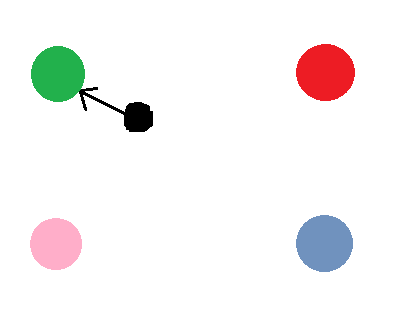
\includegraphics[width=7cm]{NN.png}
\caption{Wyszukiwanie wartości nowego piksela metodą najbliższego sąsiada}
\end{figure}

Na rysunku 1 przedstawiona jest sytuacja w której kolorem zielonym, czerwonym, różowym i niebieskim przedstawione są kolory pikseli z pewnego fragmentu obrazu źródłowego. Czarnym kołem oznaczony został nowy piksel umieszczony w odpowiadającym mu miejscu w źródłowej przestrzeni obrazu. Metoda najbliższego sąsiada dla tego piksela wynikowego wybierze kolor zielony (wskazany strzałką) z uwagi na to, że w przestrzeni źródłowej jest on najbliższy położeniu nowemu pikselowi.

Algorytm ten można stosować z powodzeniem w skalowaniu filmów o charakterystyce tak zwanego "pixel art". Jest to stylistyka wzorująca się na wyglądzie gier komputerowych z czasów, gdy dominowały platformy ośmiobitowe. Styl ten charakteryzuje się widocznymi pojedynczymi pikselami, przez co wygładzanie przejść między pikselami wynikowymi w innych algorytmach jest efektem niepożądanym. Jest to natomiast idealna sytuacja na zastosowanie algorytmu najbliższego sąsiada, jako że ten akcentuje każdy piksel powiększając go w obrazie wynikowym.

\subsubsection{Algorytm interpolacji dwuliniowej}
Algorytm interpolacji dwuliniowej polega na obliczeniu wynikowej wartości koloru na podstawie 4 pikseli otaczających.

\begin{figure}[h]
\centering
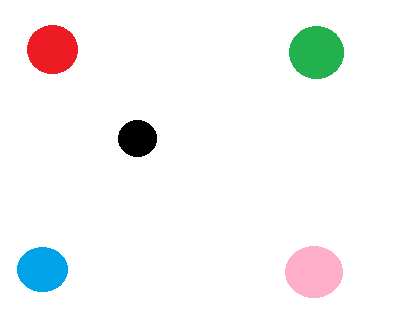
\includegraphics[width=7cm]{Interpolation1.png}
\caption{Nowy piksel w przestrzeni obrazu źródłowego}
\end{figure}

Aby obliczyć wartość koloru nowo utworzonego piksela algorytm interpolacji dwuliniowej oblicza 2 nowe piksele pośrednie. Są one wynikiem zmieszania dwóch odpowiednich pikseli (krok ten można przeprowadzić parując ze sobą piksele horyzontalnie lub wertykalnie). Mieszanie kolorów tych pikseli traktujemy jako funkcję liniową której wartości zmieniają się od jednego koloru do drugiego. Wybieramy wartość funkcji w miejscu przecięcia tej funkcji z prostą prostopadłą przechodzącą przez punkt wynikowy. W naszej implementacji wybraliśmy mieszanie horyzontalne odpowiednich kolorów.

\begin{figure}[h]
\centering
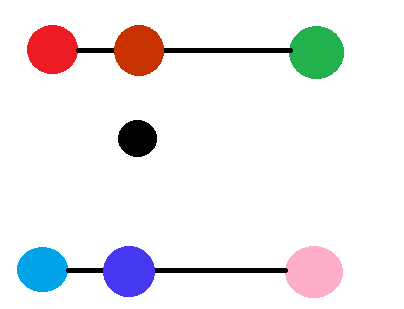
\includegraphics[width=7cm]{Interpolation2.png}
\caption{Obliczenie wartości kolorów pośrednich}
\end{figure}

Dzięki temu, otrzymane przez nas nowe piksele pośrednie znajdują się w jednej linii z pikselem wynikowym. Możemy teraz obliczyć wartość koloru piksela wynikowego używając wartości kolorów pośrednich do utworzenia nowej funkcji liniowej i wybrania jej wartości w miejscu przecięcia się funkcji z pikselem wynikowym. 

\begin{figure}[h]
\centering
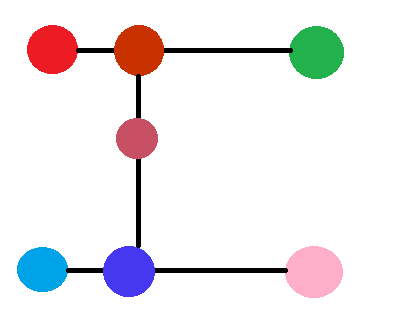
\includegraphics[width=7cm]{Interpolation3.png}
\caption{Obliczenie wartości koloru piksela wynikowego na podstawie kolorów pośrednich}
\end{figure}

Algorytm ten jest nie jest skomplikowany obliczeniowo, ale jest zauważalnie wolniejszy od algorytmu najbliższego sąsiada. Dzięki swoim właściwością, bardzo dobrze wygładza przejścia między pikselami, przez co ma szeroką gamę zastosowań.

\subsubsection{Algorytm interpolacji bikubicznej}
Algorytm ten jest najbardziej skomplikowanym obliczeniowo algorytmem jaki zaimplementowaliśmy. Korzysta on z krzywych obliczanych na podstawie macierzy pikseli rozmiaru 4 na 4. Podobnie jak w interpolacji obliczane są wartości kolorów pikseli pośrednich obliczanych dla kolejnych wierszy macierzy dzięki którym obliczany jest splajn zgodny ze wzorem Catmulla-Roma:

$sp(p_{x-1},p_x,p_{x+1},p_{x+2}) = 
\begin{bmatrix}
	1 & u & u^2 & u^3 \\[0.3em]
\end{bmatrix}
*
\begin{bmatrix}
	0 & 1 & 0 & 0 \\[0.3em]
	-\frac{1}{2} & 0 & \frac{1}{2} & 0 \\[0.3em]
	1 & -\frac{5}{2} & 2 & -\frac{1}{2} \\[0.3em]
	-\frac{1}{2} & \frac{3}{2} & -\frac{3}{2} & \frac{1}{2} \\[0.3em]
\end{bmatrix}
*
\begin{bmatrix}
	p_{x-1} \\[0.3em]
	p_x \\[0.3em]
	p_{x+1} \\[0.3em]
	p_{x+2} \\[0.3em]
\end{bmatrix}
$
\\
gdzie $u$ jest stosunkiem umiejscowienia nowego punktu na splajnie, a punkty $p_x$ są kolejnymi punktami z macierzy tworzącymi splain.

Obliczone na podstawie powyższego wzoru punkty wykorzystujemy do obliczenia ostatecznej krzywej która w miejscu przecięcia się z punktem końcowym daje nam ostateczną wartość koloru. 

\subsection{Algorytm splotu}
Algorytm splotu oblicza wartość piksela obrazu docelowego jako sumę wartości piksela znajdującego się na tej samej pozycji oraz wartości pikseli sąsiadujących z nim przemnożonych przez wartości macierzy $MxM$ zwanej maską lub kernelem. Działanie to można zapisać w następujący sposób: 
\[p_{o}[x,y]= \sum_{a = -R}^{R}\sum_{b = -R}^{R} p_{i}[x + a, y + b]*kernel[a, b]\], gdzie:

$p_{o}$ - wartość piksela obrazu wyjściowego,

$p_{i}$ - wartość piksela obrazu wejściowego,

$kernel$ - macierz maski,

$R$ - promień maski.

W naszym programie algorytm ten stosowany jest do wyostrzenia obrazu. Stosujemy do tego celu maskę: 
\[
\begin{bmatrix}
	0 & -1 & 0\\[0.3em]
	-1 & 5 & -1\\[0.3em]
	0 & -1 & 0\\[0.3em]
\end{bmatrix}
\]

\subsubsection{Obsługa pikseli brzegowych}
Algorytm splotu wymaga wartości pikseli znajdujących się poza granicami obrazu źródłowego. W tym wypadku stosuję się jedno z poniższych rozwiązań
\begin{enumerate}
	\item Obcinanie - jeżeli algorytm wymagałby do obliczenia piksela wartości znajdujących się poza krawędziami obrazu, piksel ten jest pomijany,
	\item Zawijanie - jeżeli wymagany jest piksel znajdujący się poza krawędziami obrazu, wartości te brane są z krawędzi przeciwnej,
	\item Rozszerzanie - krawędzie obrazu wejściowego rozszerzane są poprzez kopiowanie wartości pikseli brzegowych tyle razy ile wymaga tego algorytm.
\end{enumerate}

\subsection{Zwiększanie ilości klatek na sekundę}
Algorytmy zwiększające ilość klatek obrazu na sekundę są zwykle o wiele bardziej skomplikowane od algorytmów ulepszających pojedynczą klatkę obrazu. Aby stworzyć nową klatkę obrazu z dużym oddaniem tego, jak by wyglądała w rzeczywistości wymagana by była złożona analiza wielu obrazów oraz rozwiązania korzystające z systemów opartych o sztuczną inteligencję. Stworzenie pojedynczego systemu takiego rodzaju mogłoby być tematem na osobna pracę naukową. Postanowiliśmy więc skupić się na dwóch podstawowych algorytmach które dają zadowalający efekt przy użyciu prostych technik oraz niedoskonałości ludzkiego zmysłu wzroku.

\subsubsection{Algorytm interpolacji}
Algorytm interpolacji polega na tym, że klatki pośrednie tworzone są na podstawie oryginalnych klatek poprzez porównywanie dwóch klatek pomiędzy którymi ma znajdować się nowo utworzona klatka. Wartość koloru w pikselach nowo utworzonej klatce obliczana jest poprzez potraktowanie pikseli klatek oryginalnych jako funkcji liniowej której parametrem jest czas. Dzięki temu każdy piksel jest obliczany na podstawie informacji kiedy (w stosunku do dwóch oryginalnych klatek) nowa klatka się pojawia.

\begin{figure}[h]
\centering
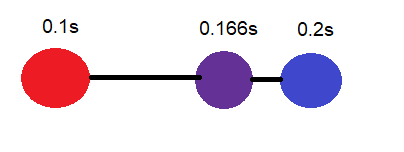
\includegraphics[width=7cm]{FpsInterpolation.png}
\caption{Obliczenie wartości koloru wynikowego na podstawie czasu}
\end{figure}

W szybko zmieniających się, dynamicznych scenach efekt ten może być widoczny jako wyraźne rozmycie, jednakże przy scenach na których nie ma gwałtownych zmian poprawia on płynność obrazu bez widzialnego negatywnego efektu.

\subsubsection{Algorytm przeplotu}
Algorytm przeplotu polega na oszukiwaniu ludzkiego oka poprzez wyświetlanie tylko połowy nowych linii. Wynikiem takiego algorytmu jest film z podwojoną ilością klatek na sekundę. Powinien on być stosowany tylko dla obrazów mających stosunkowo dużą ilość klatek na sekundę z uwagi na to, że im mniejsza jest ilość klatek na sekundę tym bardziej przeplot jest widoczny. Algorytm ten stosowano już w telewizji analogowej z uwagi na niską prędkość przesyłu oraz migotanie ekranu przy wyświetlaniu obrazu w 24 lub 30(29,97) klatkach na sekundę (odpowiednio standardy PAL oraz NTSC). Naprzemienne aktualizowanie wartości wierszy nieparzystych i parzystych obrazu przy odpowiedniej szybkości wyświetlania zwiększa wrażenie płynności obrazu, jednakże im mniejsza jest źródłowa ilość klatek na sekundę tym bardziej widoczny jest przeplot.

\begin{figure}[h]
\centering
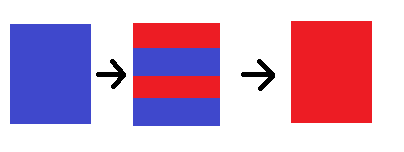
\includegraphics[width=7cm]{Interlace.png}
\caption{Tworzenie klatek pośrednich przy użyciu algorytmu przeplotu}
\end{figure}

\section{Optymalizacja i testowanie}
W implementacji algorytmów ich szybkość działania jest równie ważna co ich poprawność. W trakcie implementacji algorytmów oraz ich testowania zauważyliśmy, że ich wydajność nie była zbliżona do oczekiwanej. Przeprowadziliśmy więc szereg prac optymalizacyjnych w trakcie testowania algorytmów
\subsection{Procedura testowania i ich organizacja}
Procedura testowania jaką założyliśmy polegała na organizacji wszystkich testów w klasie TestClassModule. Testy przez nas przeprowadzane były przeprowadzane poprzez metodę RunAllToFileTests. Uruchamiała one wszystkie metody testujące głównie algorytmy ulepszające jakość pojedynczej klatki, z uwagi na to, że test taki jest prosty do zweryfikowania w aspekcie jego poprawności poprzez porównanie pojedynczej klatki wynikowej ze źródłową. Testowaliśmy także prędkość przetwarzanej klatki.

Procedurę testowania można sprowadzić do głównej części testu skupiającej się aspekcie szybkości i następnie poprawności poprzez porównanie zapisanej klatki zgodnie z formą w jakiej chcieliśmy ją zapisać - obraz, rozpisanie pikseli na tekst oraz wyświetlenie jej przy użyciu panelu w programie.

\begin{verbatim}
    int iterations = 1000;
    clock_t begin = clock();
    for (int xd = 0; xd < iterations; ++xd) {
        delete enhancer->ReadNextEnhancedFrame();
    }
    clock_t end = clock();
    double elapsed_secs = (double(end - begin)/iterations) / CLOCKS_PER_SEC;
    saveFile << std::to_string(elapsed_secs) + " sekund dla " + 
    std::to_string(iterations) +" iteracji, \n";
\end{verbatim} 

Dla 1000 iteracji pętli testujemy prędkość algorytmu przy przetwarzaniu jednej klatki obrazu. Mierzymy czas jaki zajmuje procesorowi przetworzenie 1000 klatek i dzielimy to przez ich ilość dostając względnie dokładną estymację, jak szybko przetwarzane są klatki.
Następnie zapisujemy tą wartość do pliku tekstowego.

\subsection{Optymalizacja algorytmów i układu danych}
Pierwszy i największy proces optymalizacji przeprowadziliśmy na klasie NNFrameEnhancer. Algorytm najbliższego sąsiada używany do skalowania klatki w tej klasie jest najszybszym zaimplementowanym przez nas algorytmem. Jednakże podczas pierwszego testu prędkość przetworzenia jednej klatki była liczona w minutach. Dzięki możliwości przechodzenia krok po kroku w programie Visual Studio oraz informacji, ile minęło od poprzedniego kroku udało nam się ustalić, że zastosowana dla uproszczenia kodu zmienna tymczasowa kopiowała pamięć klatki. Zauważyliśmy to dlatego, że operacja przypisania trwałą tam około 35 milisekund, gdy reszta pętli wykonywana była w kilka cykli procesora (ułamki milisekund). Usunięcie tej zmiennej przyśpieszyło program z około 14 sekund na jedną linię obrazu do 2 sekund na całą klatkę.

Niestety dalej było to o wiele za dużo względem tego czego oczekiwaliśmy po prędkości algorytmu (oczekiwaliśmy co najmniej kilkunastu klatek na sekundę). Następnymi podjętymi przez nas krokami było uproszczenie algorytmu poprzez usunięcie niektórych niepotrzebnych obliczeń. Uzyskaliśmy dzięki temu około $40\%$ przyśpieszenie. 

Następnie zmieniliśmy typ przechowywanych danych z QColor* na zwykłe wartości całkowite int. Po tych zmianach otrzymaliśmy wydajność na poziomie około 0.9 sekundy na klatkę obrazu. 

Naszym następnym krokiem była zmiana struktury danych w której przechowywaliśmy dane odnośnie pikseli. Używana przez nas struktura \begin{verbatim} boost::multi_array \end{verbatim} korzystała z 3 wymiarowej indeksacji. Zgodnie z tym co przeczytaliśmy w dokumentacji, klasa ta miała przechowywać dane w jednym, ciągłym bloku pamięci. Poprzez zmianę tej struktury na zwykłą tablicę int* uzyskaliśmy 30 krotne przyśpieszenie w przetwarzaniu danych (z 0.9 s do 0.03 s na klatkę).

Uzyskana przez nas prędkość przetwarzania była zgodna z naszymi oczekiwaniami. Postanowiliśmy zatem skorzystać z przetwarzania danych z użyciem wielu wątków. Poprzez podział danych do przetworzenia na części zgodne z ilością wątków uzyskaliśmy dodatkowe przyśpieszenie. Z uwagi na koszt utworzenia wątków najlepsze wyniki uzyskaliśmy dla 2 wątków (czas przetwarzania klatki wynosił około 0.025 sekundy). 

\begin{verbatim}
    int threads = 2;
    std::thread *tt = new std::thread[threads];

    for(int t = 0; t < threads; ++t)
    {
        tt[t] = std::thread(CalculateFramePararel, inputFrame, outputFrame,
        (_targetQualityInfo->Height / threads) * t, 
        (_targetQualityInfo->Height / threads) * (t + 1),
        _sourceQualityInfo, _targetQualityInfo);
    }

    for (int t = 0; t < threads; ++t)
    {
        tt[t].join();
    }
\end{verbatim}

Dodatkowo postanowiliśmy czytać następną klatkę źródłową w trakcie przetwarzania obecnej (jeśli jest to możliwe). Spowodowało to, że ostatecznie prędkość z jaką przetwarzamy klatki metodą najbliższego sąsiada wynosi około 0.02 sekundy, co daje nam możliwość przerabiania około 50 klatek na sekundę. Jest to wynik bardzo nas satysfakcjonujący.
%\dodatek{Mój specjalny dodatek}

%Tu treść dodatku. Zwróćmy uwagę na sposób numerowania dodatku, 
%możliwa jest zmiana numerowania, patrz wyjaśnienia.
          
%% to wpisuje się do spisu treści, ale bez numeru rozdziału,
%% można też używać \dodatek{Tytuł}, który jest numerowany, ale inaczej niż rozdziały.
%%\dodatkowo{Rysunki}

%%Tu rysunki

\begin{thebibliography}{12}

\bibitem{PozNazwa1} Jakaś pozycja literatury
\bibitem{InnPoz} Jakaś pozycja literatury

\end{thebibliography}
\end{document}
